\section{The Julia Language} \label{julia}
Julia is a dynamic scientific programming language which aims for end-to-end throughout, rather latency.
It has function-level just-in-time compilation via LLVM, and uses stable, highly-performant numeric computation libraries written in FORTRAN.

\subsection{Julia's Garbage Collector}
Julia's garbage collector uses a mark-and-sweep algorithm.
Although Julia itself can use multiple threads during normal execution, for garbage collection, it is single-threaded.
It does some pre-mark work concurrently, but in general, it is stop-the-world, meaning it waits until all threads have reached a safe point to pause, then begins garbage collection on a single thread.
It uses two generations for marking, ``young'' and ``old'', and has two type of collections, ``quick'' and ``full'', which involve collecting just the young generation or the entire mass of memory, respectively.

An new object begins life in the young generation, with its mark bit initially set to clean.
During any garbage collection (quick or full), if it is marked and hasn't survived some arbitrary number of collections, it is returned to a clean state and persists for further use by the program.
If it is marked and is old enough to be promoted, it is marked as old.
During subsequent full collections, when this old object is marked, its mark bit gets changed once again to be identifiable as being both old and marked, and a write barrier is set up so that it can remembered in the remembered set if it points to young objects.

Each program thread maintains its own set of thread-local object pools, categorized by size, for allocating small objects.
Big objects, however, are allocated with \texttt{malloc} and are consequently stored on global big object lists.
It doesn't impose a maximum heap size, requesting a very large heap from the OS initially and thus relying on overcommitting.
Because of the lack of bounds on heap size, garbage collection kicks in on dynamic periods, because there is no internal out-of-memory limit to rely on.

\subsection{Julia's Page Manager}
Julia uses it own page manager for memory allocation.
It allocates pages via the \texttt{mmap} system call, organizing these pages into 32-page chunks and likewise these chunks into N-chunk regions.
Each region tracks which chunks of pages are allocated via an allocation map, which is an N-length array storing 32-bit bitmaps representing each page within a chunk.
This way, Julia can track which pages have young data or marked objects, making checking during the sweep phase quick because only a single bit needs to be checked in order to skip a page.

\subsection{GC Stages}
\begin{figure}[h]
  \centering
  \begin{subfigure}{0.45\textwidth}
    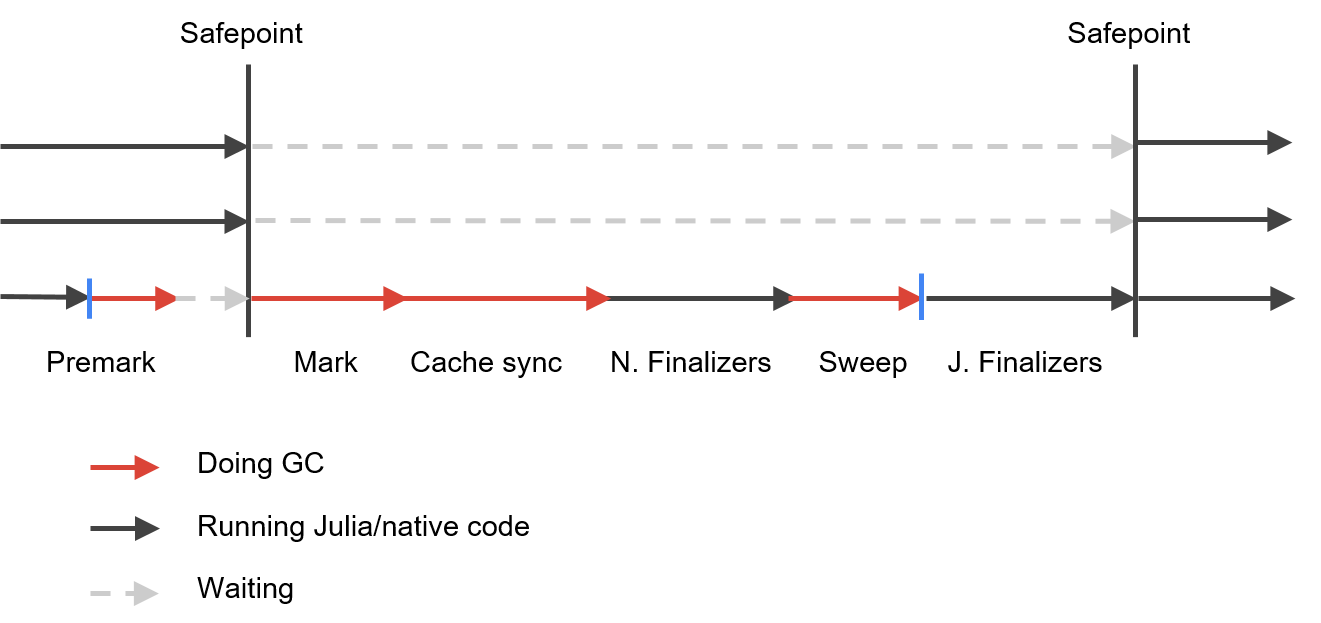
\includegraphics[width=\textwidth]{julia-gc.png}
    \caption{Stages of Julia GC}
    \label{fig:stages:jl}
  \end{subfigure}
  \begin{subfigure}{0.45\textwidth}
    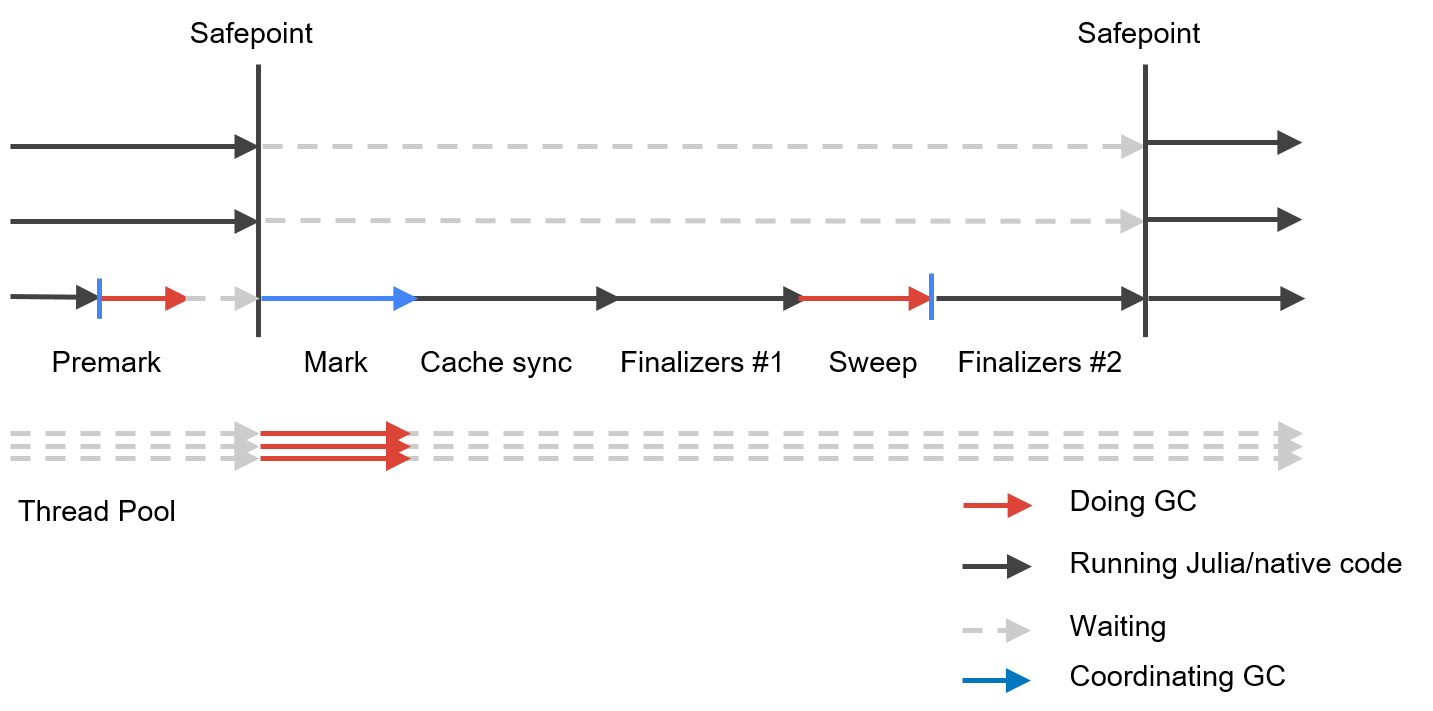
\includegraphics[width=\textwidth]{neptune-gc.png}
    \caption{Stages of Neptune GC}
    \label{fig:stages:np}
  \end{subfigure}
  \caption{Stages of Julia GC and Neptune}
  \label{fig:stages}
\end{figure}

Figure \ref{fig:stages:jl} shows the various stages of Julia's garbage collection.
Julia begins garbage collection choosing a thread to the collection.
This thread acquires the global GC lock and begins doing some premarking work concurrently with other program threads, which soon learn that they must stop normal execution because garbage collection is going to begin.

Once all the threads have suspended normal execution and reached a safe point, the GC begins the process of marking.
Marking is the process of traversing the root set and all objects recursively reachable from said root set in order to mark all memory in use as actually in use.
Specifically, it first marks all pointer-free objects (the empty tuple type, \textbf{true}, \textbf{false}, etc.).
Then it marks each thread's remembered set objects (i.e. all old objects that point to younger ones, which were remembered from the last garbage collection).
Next it marks each thread's local roots (the thread's modules, tasks, etc.).
It also marks the initial root set (built-in values, assorted constants, etc.) and objects referenced by objects on the finalizer lists.
Finally, it marks objects put on the mark stack during the previous marking process just described, because of an imposed marking depth limit.

The process of marking an individual object is fairly straightforward.
The collector first checks the current recursion depth, queuing the object if too high.
Otherwise, it essentially performs a large switch-case statement on the object's type tag.
If it is a vector or array, it marks and recursively scans the object's vector/array contents.
If the object is a user data type, it marks and scans its fields; and similarly for other objects.

After marking, the Julia GC flushes the mark cache, which involves moving big objects in the a big object cache to the corresponding big objects list so subsequent sweeping can see them.
It also then causes native finalizers to run.

Once flushed, the collector begins the sweep phase.
Sweeping is the process of traversing all of memory and reclaiming the space previously used by unmarked (i.e. unreachable and therefore garbage) objects.
Specifically, Julia's GC sweeps the finalizer list (at the same time scheduling objects for finalization), weak references, malloc'ed arrays, big objects, and each pool in each thread.

Finally, the collector thread releases its hold of the global GC lock, calling the Julia finalizers.
Once completed, it causes all threads suspended at their safe points to resume normal execution.

% TODO probably redo graphics to look better?
%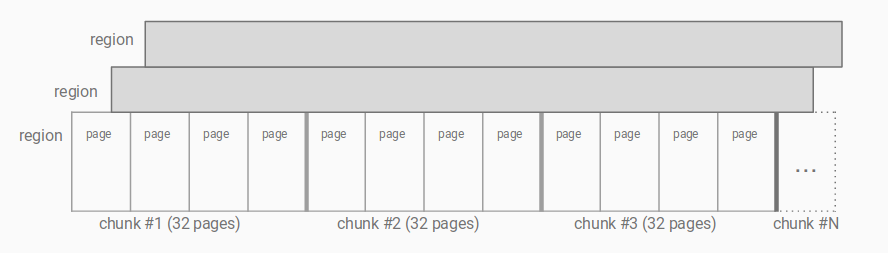
\includegraphics{regions}
%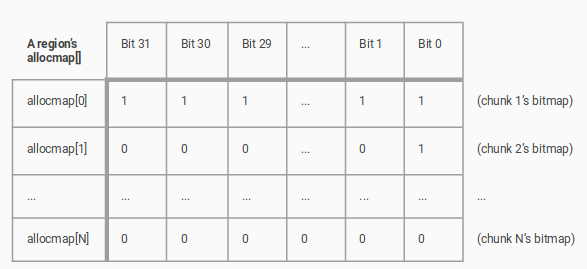
\includegraphics{allocmap}
%\includegraphics{stages}

%%% Local Variables:
%%% mode: latex
%%% TeX-master: "report"
%%% End:
